\section*{Microeconomics Midterm 2015 / 16}

{
\subsection*{Schmidt}

\subsubsection*{Exercise 1}

\begin{enumerate}[label=(\alph*)]
{\item 
To violate WARP:

find $w$ by Walras law

$$
\begin{aligned}
& \left|\begin{array}{l}
p^{\prime} y \leqslant w^{\prime} \\
p y^{\prime} \leqslant w
\end{array}\right| \\
\Leftrightarrow&\left|\begin{array}{l}
30(12+x) \leqslant 600 \\
10(30+24) \leqslant 360+24 x
\end{array}\right| \\
\Leftrightarrow& \left|\begin{array}{l}
30 x \leqslant 240 \\
180 \leqslant 24 x
\end{array}\right| \\
\Leftrightarrow& \left|\begin{array}{l}
30 x \leqslant 240 \\
180 \leqslant 24 x
\end{array}\right| \\
\Leftrightarrow& \left|\begin{array}{c}
x \leqslant 8 \\
7.5 \leqslant x
\end{array}\right|
\end{aligned}
$$

WARP is violated for $x \in[7.5,8]$.
}
{\item
Bundle 2 must be affordable in period 1. Then we see that the consumer chooses bundle 1 over bundle 2: $x \leqslant 8$ by (a)

To not violate WARP we find that if and only if $x \in[0,7.5)$, bundle 1 is revealed preferred.
}
{\item 
The quantity increased. To have an inferior good, $\frac{\partial y_{1}}{\partial w}<0$. Thus, income must have decreased:

$$
\begin{aligned}
600 & \leqslant 360+24 x \\
\Leftrightarrow 10 & \leqslant x
\end{aligned}
$$

We find that good 1 is inferior for $x \geqslant 10$.
}
\end{enumerate}
}
{
\subsubsection*{Exercise 2}

Monotone transformation to $u_{2}(\cdot)$ :

$$
\tilde{u}_{2}\left(x_{1}, x_{2}\right)=x_{1}^{\frac{3}{3+a}} x_{2}^{\frac{a}{3+a}}
$$

\begin{enumerate}[label=(\alph*)]
{\item
consumer 1: Invert $e_{1}(\cdot)$. In equilibrium $e_{1}(\cdot)=w_{1}$ and $v_{1}\left(p, w_{1}\right)=u_{1}$ :

$$
\begin{aligned}
& w_{1}=v_{1}\left(p, w_{1}\right) \sqrt{p_{1} p_{2}} \\
\Leftrightarrow \quad & v_{1}\left(p, w_{1}\right)=\frac{w_{1}}{\sqrt{p_{1} p_{2}}}
\end{aligned}
$$

Apply Roy's identity:

$$
x_{1}^{1}\left(p_{1}, w_{1}\right)=-\frac{\frac{\partial v_{1}(\cdot)}{\partial p_{1}}}{\frac{\partial v_{1}(\cdot)}{\partial w}}=-\frac{-\frac{1}{2} p_{1}^{-3/2} \frac{w}{\sqrt{p_{2}}}}{\frac{1}{\sqrt{p_{1} p_{2}}}}
$$

$$
x_{1}^{1}\left(p_{1}, w_{1}\right)=\frac{1}{2} \frac{w_{1}}{p_{1}}
$$

By symmetry of $v_{1}\left(p, w_{1}\right)$ :

$$
x_{2}^{1}\left(p_{1}, w_{1}\right)=\frac{1}{2} \frac{w_{1}}{p_{2}}
$$

consumer 2: As $\tilde{u}_2(\cdot)$ is standard Cobb-Douglas, the result is immediate:

$$
\begin{aligned}
& x_{1}^{2}\left(p, w_{2}\right)=\frac{3}{3+a} \frac{w_{2}}{p_{1}} \\
& x_{1}^{2}\left(p, w_{2}\right)=\frac{a}{3+a} \frac{w_{2}}{p_{2}}
\end{aligned}
$$
}
{\item 
Aggregate demand: $x_{l}=x_{l}^{1}+x_{l}^{2}$

Good 1: $x_{1}=\frac{1}{p_{1}}\left[\frac{1}{2} w_{1}+\frac{3}{3+a} w_{2}\right] \rightarrow \frac{1}{2} \stackrel{!}{=} \frac{3}{3+a}$

Good 2: $x_{2}=\frac{1}{p_{2}}\left[\frac{1}{2} w_{1}+\frac{a}{3+a} w_{2}\right] \rightarrow \frac{1}{2} \stackrel{!}{=} \frac{a}{3+a}$

In both cases: $a=3$
}
\end{enumerate}
}
{
\subsubsection*{Exercise 3}

\begin{enumerate}[label=(\alph*)]
{\item
$R=-C V$ as it is the amount that has to be given after implementing the change.

The Leontief preferences imply that they must be able to afford the old bundle \& they will buy it.

By Leontief: $\quad x_{1}=x_{2} \rightarrow w=\left(p_{1}+p_{2}\right) x_{1}$

Before moving: $\quad 1000=2 \cdot x_{1} \Leftrightarrow x_{1}=x_{2}=500$

After moving: $1000+R=5 \cdot x_{1} \Leftrightarrow R=5 x_{1}-1000$

As discussed, must choose same bundle to have $u_{0}=u_{1}=500$.

$$
R=2500-1000=1500
$$
}
{\item 
Cobb-Daglas implies: $x_{l}=\frac{1}{2} \frac{w}{p_{l}}$

Before moving:

$$
x_{1}=x_{2}=500 \rightarrow u_{0}=500
$$

After moving:

$$
\begin{aligned}
& x_{1}=\frac{1}{2} \frac{(1000+R)}{4} \\
& x_{2}=\frac{1}{2}(1000+R) \\
& u_{1}=\frac{1000+R}{2} \frac{1}{2} \stackrel{!}{=} u_{0}=500 \\
& \Leftrightarrow R=1000
\end{aligned}
$$

We plug $R$ into demands: $x_{1}=250 ;\: x_{2}=1000$.

The demand for $x_{1}$ decreased and it increased for $x_{2}$. Reason being that Cobb-Douglas (unlike Leontief) allows for substitution. Therefore, demand followed the price change.
}
\end{enumerate}
}

\newpage
{
\subsection*{Gottardi}

\subsubsection*{Exercise 1}

Only relative prices matter. Define $p^{\text {aut }}=\frac{p_{1}^{\text {aut }}}{p_{2}^{\text {aut }}}$ and $p=\frac{p_{1}}{p_{2}}$.

\underline{Case 1:} ( $\left.p=p^{\text {aut }}\right)$

Nothing changes. No welfare effects.

\underline{Case 2:} ( $p>p^{\text {aut })}$

Assume A sells commodity 1. Then the price increase benefits her, as she can sell at a higher price.

Assume A buys commodity 1. The effect depends on her ability to substitute, which depends on her preferences. There three three options:

(i) She switches to selling commodity 1. The price change is beneficial.

(ii) She can substitute without gaining from it in terms of utility.

(iii) She cannot substitute sufficiently and the price change hurts her.

The graphs illustrate the three cases. Green are equilibria. 1 is under autarky \& 2 after opening p. Blue are budget sets \& pink are indifference curves.

\begin{figure}[!h]
    \centering
    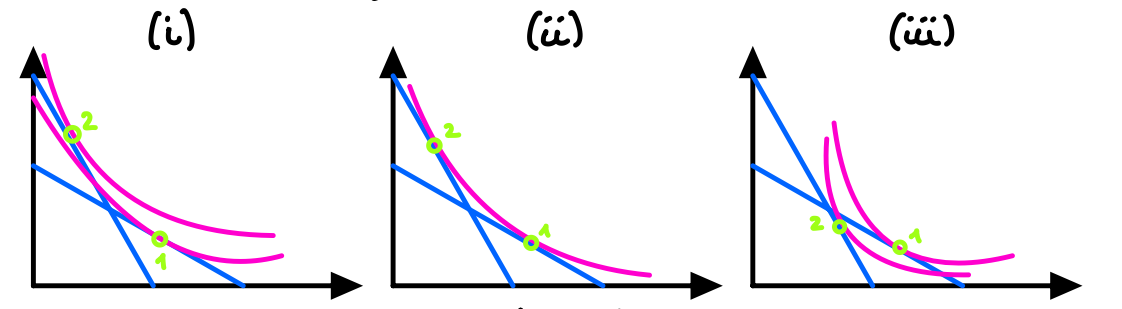
\includegraphics[width=\textwidth]{images/2015_16_1.png}
\end{figure}

\underline{Case 3:} ( $\left.p<p^{\text {aut }}\right)$

Substitute $A$ sells 1 and buys 1 in case 2. The argument is just the inverse.

For agent $B$ the argument is always just the inverse in all cases.

We see that at least one agent is weakly better off.
}
{
\subsubsection*{Exercise 2}

\begin{enumerate}[label=(\alph*)]
{\item
Since $A$ cares more about $x_{1}$ and $B$ more about $x_{2}$, the PE allocations ce around the edges of the box (in blue).

$$
P E=\left\{x_{2}^{A}=0 \text{ or } x_{1}^{B}=0\right\}
$$

\begin{figure}[!h]
    \centering
    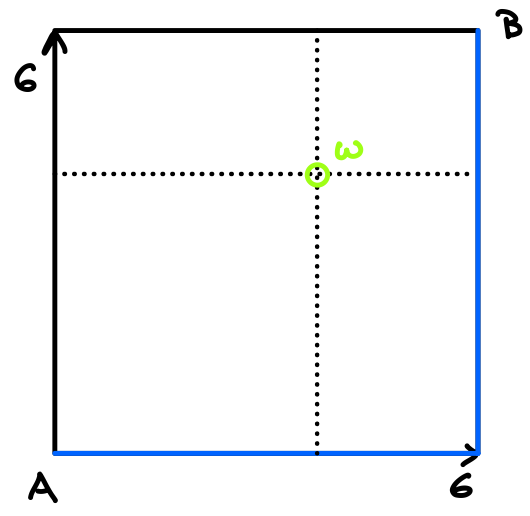
\includegraphics[width=.5\textwidth]{images/2015_16_2.png}
\end{figure}
}
{\item
For PE, equate MRS across agents:

$$
\operatorname{MRS}^{A}=2 \stackrel{!}{=} \operatorname{MRS}^{B}=\frac{x_{2}^{B}}{x_{1}^{B}} \Leftrightarrow x_{2}^{B}=2 x_{1}^{B}
$$

For $C E$ consumers behave optimally \& markets must clear. Let $p=p_{1} / p_{2}$

A: By linearity of preferences:

$$
x_{1}^{A}=\left\{\begin{array}{lll}
    \infty & \text {if } p<2 \\
    \mathbb{R}^{+} & \text {if } p=2 \\
    0 & \text {if } p>2
\end{array} \quad x_{2}^{A}=\left\{\begin{array}{lll}
    \infty & \text {if } p>2 \\
    \mathbb{R}^{+} & \text {if } p=2 \\
    0 & \text {if } p<2
\end{array}\right.\right.
$$

B:

\begin{align*}
    \max _{C_{1}^{8}, c_{2}^{8}} \ln \left(x_{1}^{8}\right)+\ln \left(x_{2}^{8}\right) \\
    \text{s.t. } p x_{1}^{B}+x_{2}^{B}=p^{2}+2
\end{align*}

FOCs

\begin{align*}
    &\frac{1}{x_{1}^{B}}-\lambda p=0 \\
    &\frac{1}{x_{2}^{B}}-\lambda=0 \\
    \Longrightarrow \quad & x_{2}^{B}=x_{1}^{B} p
\end{align*}

Plug into $B C$ :

$$
x_{1}^{B}=\frac{p+1}{p} ; x_{2}^{B}=p+1
$$

\underline{Market Clearing: } 

For markets to clear we have $p=2$. Otherwise $A$ will have infinite demand for one of the goods:

$$
\begin{gathered}
x_{1}^{B}=\frac{3}{2} ;\quad x_{2}^{B}=3 \\
x_{1}^{A}=6-x_{1}^{3}=\frac{9}{2} ;\quad x_{2}^{A}=6-x_{2}^{B}=3
\end{gathered}
$$

\underline{Competitive Equilibrium: }

\begin{align*}
    \left(x_{1}^{A}, x_{2}^{A}\right) &= (\frac{9}{2},3) \\
    \left(x_{1}^{B}, x_{2}^{B}\right) &= (\frac{3}{2},3) \\
    p&=2
\end{align*}

It is $P E$ since $x_{2}^{B}=3=p x_{1}^{B}=2\frac{3}{2}$.
}
\end{enumerate}
}
{
\subsubsection*{Exercise 3} % continue here

$$
w^{A}=(8,4) ; w^{B}=(2,4)
$$

\begin{enumerate}[label=(\alph*)]
{\item
$$
\begin{aligned}
& M R S^{A}=\frac{1 / 2}{1 / 2}=1 \stackrel{!}{=} MRS^{B}=\frac{1 / 2}{1 / 2} \frac{\frac{\partial u^{B}(\cdot)}{\partial x_{1}}}{\frac{\partial u^{B}(\cdot)}{\partial x_{2}}} \\
& \Longleftrightarrow \frac{\partial u^{B} \left(\cdot\right)}{\partial x_{1}}=\frac{\partial u^{B}(\cdot)}{\partial x_{2}} \Longleftrightarrow x_{1}^{B}=x_{2}^{B}
\end{aligned}
$$

PE in blue. Defined by

$$
x_{2}^{B}=\left\{\begin{array}{ll}
x_{1}^{B} & \text { if } x_{1}^{B} \leq 8 \\
8 & \text { else }
\end{array}\right\}
$$

\begin{figure}[!h]
    \centering
    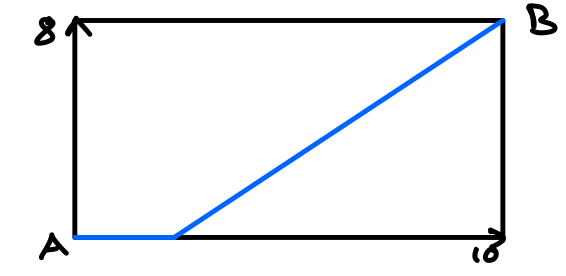
\includegraphics[width=.5\textwidth]{images/2015_16_3.png}
\end{figure}
}
{\item 
Budget constraints:

\begin{align*}
    \text{at } t = 0: \quad & q_1 \theta_1^h+q_2 \theta_2^h=0 \\
    \text{at } t = 1: \quad & x_1^h=w_1^h+\theta_1^h \\
    & x_2^h=w_2^h+\theta_2^h
\end{align*}

Plug the $\theta$s into first BC:

$$
q_{1}\left(x_{1}^{h}-w_{1}^{h}\right)+q_{2}\left(x_{2}^{h}-w_{2}^{h}\right)=0
$$

UMP:

$$
\begin{aligned}
& \max _{x_{1}^{h}, x_{2}^{h}} \quad \pi_{1} u^{h}\left(x_{1}^{h}\right)+\pi_{2} u^{h}\left(x_{2}^{h}\right) \\
& \text { s.t. } q_{1}\left(x_{1}^{h}-w_{1}^{h}\right)+q_{2}\left(x_{2}^{h}-w_{2}^{h}\right)=0
\end{aligned}
$$

FOCs:

\begin{align*}
    \pi_{1} \frac{\partial u^{h}(\cdot)}{\partial x_{1}^{h}}-\lambda q_{1}=0 \\
    \pi_{2} \frac{\partial u^{h}(\cdot)}{\partial x_{2}^{h}}-\lambda q_{2}=0 \\
    \longrightarrow \frac{q_{1}}{q_{2}}=\frac{\pi_{1}}{\pi_{2}} \frac{\partial u^{h}(\cdot)}{\partial x_{1}^{h}}\left(\frac{\partial u^{h}(\cdot)}{\partial x_{2}^{h}}\right)^{-1} \tag{I}
\end{align*}

\underline{Agent A:}

By $\pi_{1}=\pi_{2}$ \& linearity:

\begin{align*}
    \frac{q_{1}}{q_{2}}=1
\end{align*}

\underline{Agent B:}

Plug $\frac{q_{1}}{q_{2}}=1$ into (I) and also $\pi_{1}=\pi_{2}$ :

\begin{equation*}
    \frac{\partial u^{B}(\cdot)}{\partial x_{1}^{B}}=\frac{\partial u^{B}(\cdot)}{\partial x^{3}} \Leftrightarrow x_{1}^{B}=x_{2}^{B} \tag{II}
\end{equation*}

Plug (II) into $B C$ of $B$ using $\frac{q_{1}}{q_{2}}=1$ :

$$
x_{1}^{B}=x_{2}^{B}=\frac{w_{1}^{B}+w_{2}^{B}}{2}=3
$$

\underline{Market Clearing: }

$$
\begin{aligned}
& x_{1}^{A} \stackrel{!}{=} w_{1}^{A}+w_{1}^{B}-x_{1}^{B}=7 \\
& x_{2}^{A} \stackrel{!}{=} w_{2}^{A}+w_{2}^{B}-x_{2}^{B}=5
\end{aligned}
$$

\underline{Competitive Equilibrium: }

$$
\begin{aligned}
\left(x_{1}^{A}, x_{2}^{A}\right) & =(7,5) \\
\left(x_{1}^{B}, x_{2}^{B}\right) & =(3,3) \\
\frac{q_{1}}{q_2} & =1
\end{aligned}
$$

It is PE as $x_{1}^{B}<8$ and $x_{2}^{B}=x_{1}^{B}$.
}
{\item 
By (I) we know that $\frac{q_{1}}{q_{2}}>1$. Thus insurance for $B$ is more expensive $\&$ she buys less of it. At the same time, $A$ believes $s=1$ to be more likely. Therefore, $A$ consumes more in $s=1$, and $B$ less. A consumes less in $s=2, B$ consumes more.
}
\end{enumerate}
}